\documentclass[12pt,letterpaper,noanswers]{exam}
\usepackage[usenames,dvipsnames,svgnames,table]{xcolor}
\usepackage[margin=0.9in]{geometry}
\renewcommand{\familydefault}{\sfdefault}
\usepackage{multicol}
\usepackage{wrapfig}
\pagestyle{head}
\header{AM 22b Class 36}{}{Apr 26: Differential equations, p.\thepage}
\runningheadrule
\headrule
\usepackage{graphicx} % more modern
\usepackage{amsmath} 
\usepackage{amssymb} 
\usepackage{hyperref}
\usepackage{tcolorbox}
\usepackage[utf8]{inputenc}
\usepackage{diagbox}
\usepackage{graphicx} 
\usepackage{enumitem}
\usepackage{tikz}
\tikzstyle{startstop} = [rectangle, rounded corners, minimum width=3cm, minimum height=1cm,text centered, draw=black]

\tikzstyle{process} = [rectangle, minimum width=3cm, minimum height=1cm, text centered, draw=black, fill=gray!20]
\tikzstyle{decision} = [ellipse, minimum width=3cm, minimum height=0.5cm, text centered, draw=black, fill=white!30]
\tikzstyle{arrow} = [thick,->,>=stealth]
\usetikzlibrary{shapes.geometric, arrows}
\pagenumbering{arabic}

\usepackage[numbered,autolinebreaks,useliterate]{mcode}

\newcommand{\mb}[1]{\underline{#1}}

\begin{document}
 \pdfpageheight 11in 
  \pdfpagewidth 8.5in




% I need to review the torus trajectories...

\begin{itemize}
% \item There is a pre-class assignment (20 minutes of videos + a few WeBWorK exercises) due at 10am this Monday.  It is available on Canvas.
\itemsep0em
\item PSet 10 is due Thurs Apr 29th at 6pm ET.
\item Our final skill check is today.
\item If it would be helpful for you to have an alternate deadline for PSet 10, make arrangements with me via direct message on Slack.
\item Quiz 07 (our final assignment) will be available from May 8th at 5pm to May 12th at 5pm.
\end{itemize}

\hrule
\vspace{0.2cm}

% partial derivatives, gradient
% local linearity, differential, directional deriv
% 2nd order partials + equations with partials

\noindent\textbf{Big picture}

We will learn how to analyze differential equations from three perspectives: using approximate solutions (slope fields + Euler's method + RK45), finding exact solutions (rarely, using separation of variables), using qualitative methods (identifying equilibrium solutions and whether they are `stable' or `unstable').

Today we will work with systems of equations.


\vspace{0.2cm}
\hrule
\vspace{0.2cm}

\noindent\textbf{Teams}

\begin{multicols}{2}

1.  student names
\end{multicols}


\vspace{0.2cm}
\hrule
\vspace{0.2cm}



 \noindent\textbf{A system of first order equations from approximating an infinite-dimensional system (time delay)}
    \begin{tcolorbox}
    \begin{itemize}
    \itemsep0em

    \item Systems of first order differential equations also arise in the process of approximating a system with time delay.  
    \begin{itemize}
    \itemsep0em
        \item $\dfrac{dP(t)}{dt} = aP(t-k)$ is an equation where the rate of change of the current population is proportional to the population at a time $k$ days ago (where $t$ is measured in days), rather than proportional to the current population.
        \item For a driver accelerating in traffic, moving in response to the motion of the car in front of them, their reaction time can be modeled via a delay.
    \end{itemize}
    \item Finding solutions for a system with delay requires techniques beyond the scope of this course.
    \item Using the delayed system, there exist related higher-order systems: for a very short time delay, a process of Taylor expanding would generate an \textbf{infinite order} differential equation.  As an approximation, this can be truncated at finite order.
    \item The truncated approximation can be transformed into a first order system, with the dimension of the system set by the degree of the truncated Taylor expansion.  The finite dimensional system that results is an approximation to an \textbf{infinite dimensional} system that would arise with no truncation.
\end{itemize}
\end{tcolorbox}
\noindent\textbf{Example. A short time delay.}

Consider $\frac{dP}{dt} = aP(t-k)$ where $k$ is small.  Use Taylor expansion.

$\frac{dP}{dt} \approx aP(t) -ak\frac{dP}{dt}(t) +ak^2 \frac{d^2P}{dt^2}/2 + ...$

Approximate the equation as $\dot P = aP - ak\dot P + \frac{ak^2}{2}\ddot P$.  Rewrite this as a first order system.

If it is linear, write the resulting system via a matrix equation.

\vspace{1.7in}


\vspace{0.2cm}
\hrule
\vspace{0.2cm}



\noindent\textbf{Linear systems: solutions}
\begin{tcolorbox}
\begin{itemize}
\itemsep0em
    \item Consider a linear, autonomous, homogeneous system written in matrix form: $\frac{d}{dt}\underline x = A \underline x$.  
    \item Let $\underline v_k$ be an eigenvector of $A$ with $\lambda_k$ the corresponding eigenvalue.  Let $\underline x_k(t) = \underline v_k e^{\lambda_k t}$.  $\underline x_k$ is a solution to the differential equation.
    \item An \textbf{eigenvector} and \textbf{eigenvalue} pair of a matrix $A$ satisfy $A\underline v = \lambda\underline v$.  $\underline v$ is a \emph{similarity vector} of the matrix (a vector where its direction is not changed under the action of the matrix) and $\lambda$ is its \emph{similarity coefficient}.
\end{itemize}
\end{tcolorbox}
\noindent\textbf{Example.  Linear system}.  

Let $\dot x = 11x - 3y, \dot y = 36x - 10y$.
\begin{enumerate}
    \item Write the system in matrix form.
    \vspace{0.7in}
    \item Find the eigenvalue, $\lambda_1$, associated with $\underline v_1 = \left(\begin{array}{c} 1 \\ 3\end{array}\right)$.
    \vspace{1in}
    \item Show that $c\underline v_1 e^{\lambda_1 t}$ satisfies the system.
    \vspace{1.5in}
    \item Find the eigenvalue, $\lambda_2$, associated with $\underline v_2 = \left(\begin{array}{c} 1 \\ 4\end{array}\right)$, and construct a second family of solutions.
    \vspace{1in}
    \item Show that a linear combination of your solutions is also a solution.
    \vspace{2in}
    \item In the phase plane (the $xy$-plane), draw flow lines that correspond to your two solutions.
    \vspace{2in}
    
\end{enumerate}


\vspace{0.2cm}
\hrule
\vspace{0.2cm}

\noindent\textbf{Straight line solutions}
\begin{tcolorbox}
\begin{itemize}
    \item For a linear system of the form $\frac{d}{dt}\left(\begin{array}{c} x \\ y \end{array}\right) = A\left(\begin{array}{c} x \\ y \end{array}\right)$, straight-line solutions occur when $A\left(\begin{array}{c} x \\ y \end{array}\right)$ points in the same (or opposite) direction as the vector from $(0,0)$ to $(x,y)$.
\item Straight-line solutions occur when there is a number $\lambda$ such that $A\left(\begin{array}{c} x \\ y \end{array}\right) = \lambda \left(\begin{array}{c} x \\ y \end{array}\right)$ (for $\lambda$ a real number).
\end{itemize}
\end{tcolorbox}

\noindent\textbf{Example}

Let $\frac{d\underline{x}}{dt} = \left(\begin{array}{c c}3 & 2 \\ 0 & -2\end{array}\right)\underline{x}$.
\begin{enumerate}
    \item Compute the eigenvalues.
    \vspace{1in}
    \item Find the associated eigenvectors.
    \vspace{1in}
    \item Plot straight line solutions (include an arrow to show the direction of motion along the solution).
    \vspace{2in}
\end{enumerate}


\vspace{0.2cm}
\hrule
\vspace{0.2cm}

\noindent\textbf{General solutions}
\begin{tcolorbox}
\begin{itemize}
    \item 
For the system $\frac{d\underline{x}}{dt} = A\underline{x}$, wth $A$ an $n\times n$ matrix, suppose $\underline{x}_1, \underline{x}_2,...,\underline{x}_n$ are $n$ solutions.  If the solutions are linearly independent, then the \textbf{general solution} to the system is $\underline{x}(t) = c_1\underline{x}_1(t) + c_2 \underline{x}_2(t) + ... + c_n\underline{x}_n(t)$.
\item Determining whether solutions are linearly independent can be done using a determinant called the \textbf{Wronskian}.  It is beyond the scope of this class (you would learn to use a Wronskian in AM105).
\end{itemize}
\end{tcolorbox}

For $\frac{d\underline{x}}{dt} = \left(\begin{array}{c c}3 & 2 \\ 0 & -2\end{array}\right)\underline{x}$, if the eigenvalues are distinct then the straight line solutions you found above are linearly independent.  Use them to construct a general solution.
\vspace{1.5in}

Let $\frac{d\underline{x}}{dt} = \left(\begin{array}{c c}-2 & -3 \\ 3 & -2\end{array}\right)\underline{x}$.  Find the eigenvalues and eigenvectors of this system, and use them to construct solutions to the differential equation.
\vspace{2in}


\vspace{0.2cm}
\hrule
\vspace{0.2cm}
\noindent\textbf{Complex-valued eigenvalues}
\begin{tcolorbox}
\begin{itemize}
    \item \textbf{Euler's formula} says that $e^{ib} = \cos b + i\sin b$.
    \item Suppose $\underline{x}(t)$ is a complex valued solution to a linear system $\frac{d\underline{x}}{dt}= A\underline{x}$.  Suppose $\underline{x}(t) = \underline{x}_{\text{re}}(t) + i\underline{x}_{im}(t)$ where $\underline{x}_{\text{re}}(t)$ and $\underline{x}_{im}(t)$ are real-valued functions of $t$.  Then $\underline{x}_{re}(t)$ and $\underline{x}_{im}(t)$ are both solutions of the original system $\frac{d\underline{x}}{dt}= A\underline{x}$.
\end{itemize}
\emph{Theorem is from Blanchard, Devaney, and Hall, section 3.4: complex eigenvalues}

\end{tcolorbox}

Construct two real solutions to the system $\frac{d\underline{x}}{dt} = \left(\begin{array}{c c}-2 & -3 \\ 3 & -2\end{array}\right)\underline{x}$.

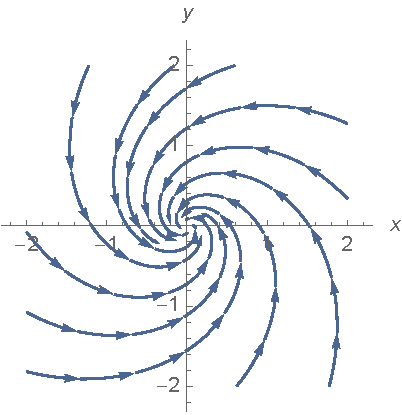
\includegraphics{img/C36phase.pdf}

\end{document}